\documentclass{beamer}

\mode<presentation>

\usetheme{Darmstadt}
\useoutertheme[footline=authorinstitutetitle]{miniframes}
\setbeamercolor{alerted text}{fg=blue}

\usepackage[brazil]{babel}
\usepackage[utf8]{inputenc}
\usepackage{amsmath}
\usepackage{float}
\usepackage{amssymb}
\usepackage{epsfig}
\usepackage{graphics}
\usepackage{graphicx}
\usepackage{amsthm}
\usepackage{mathrsfs}
\usepackage{xspace}
\usepackage{enumerate}
\usepackage[tight,raggedright]{subfigure}
\usepackage{wrapfig}
\usepackage{picinpar}
\usepackage{calc}

\def\upo{\textsuperscript{\d o}\xspace}
\def\upa{\textsuperscript{\d a}\xspace}

\def\MMe{\mathrm{e}} % constante de Euler
\def\MMi{\mathrm{i}} % constante imaginária
\def\MMd{\mathrm{d}} % diferencial total
\def\MMpi{\mathrm{\pi}}
\def\MMD{\mathrm{D}} % discrepância
\def\MMN{\mathbb{N}} % conjunto dos números naturais
\def\MMZ{\mathbb{Z}} % conjunto dos números inteiros
\def\MMQ{\mathbb{Q}} % conjunto dos números racionais
\def\MMQbar{\overline{\mathbb{Q}}} % conjunto dos números irracionais
\def\MMR{\mathbb{R}} % conjunto dos números reais
\def\MMC{\mathbb{C}} % conjunto dos números complexos
\def\Prob{\mathbb{P}} % função de probabilidades
\def\MMp{\mathrm{.}} % ponto de texto
\def\MMv{\mathrm{,}} % vírgula de texto
\def\MMpv{\mathrm{;}} % ponto-e-vírgula de texto
\def\geq{\geqslant} % desigualdade superior
\def\leq{\leqslant} % desigualdade inferior
\def\divd{\backslash} % divisão própria
\def\ndivd{\nbackslash} % divisão própria negada
\def\parenteses#1{\left( #1 \right)} % parênteses com tamanho arbitrário
\def\colchetes#1{\left[ #1 \right]} % colchetes com tamanho arbitrário
\def\chaves#1{\left\{ #1 \right\}} % chaves com tamanho arbitrário
\def\cardi#1{\lvert #1 \rvert} % cardinalidade
\def\Bigcardi#1{\Bigl\lvert #1 \Bigr\rvert}
\def\chao#1{\left\lfloor #1\right\rfloor} % chão
\def\teto#1{\left\lceil #1\right\rceil} % teto
\def\funcao#1#2#3{#1\colon #2\rightarrow #3} % definição de função
\def\cj#1{\chaves{#1}} % definição explícita de conjunto
\def\cjbar#1#2{\chaves{#1\vert#2\right.}} % conjunto com |
\def\cjpp#1#2{\chaves{#1\colon#2}} % conjunto com :
\def\galois#1{\mathbb{F}_{#1}} % corpo de Galois
\def\cquoc#1#2{{#1}_{{\displaystyle\diagup}_{\displaystyle{#2}}}}
  % conjunto quociente
\def\tcquoc#1#2{^{#1}{\scriptstyle\diagup}_{{#2}}}
  % conjunto quociente para ambientes de texto
\def\clP{\mathcal{P}}
\def\clNP{\mathcal{NP}}
\def\clBPP{\mathcal{BPP}}
\def\clcoNP{\mathsf{co}\text{-}\clNP}
\def\leqp{\leq_{\clP}}
\def\codf#1{\langle #1\rangle}
\def\vetor#1{\boldsymbol{#1}}
\def\matriz#1{\mathsf{#1}}
\def\norma#1#2{{\lVert{#2}\rVert}_{#1}}
\def\lrnorma#1#2{{\left\lVert{#2}\right\rVert}_{#1}}
\def\transp#1{{#1}^{\scriptscriptstyle \top}}
\def\foraa{\tilde{\forall}}
\def\tende{\rightarrow}
\makeatletter
  \def\sen{\mathop{\operator@font sen}\nolimits} % seno
  \def\arcsen{\mathop{\operator@font arcsen}\nolimits} % arco-cosseno
  \def\diam{\mathop{\operator@font diam}} % diâmetro
  \def\cin{\mathop{\operator@font cin}} % cintura
  \def\dist{\mathop{\operator@font dist}} % distância
  \def\ord{\mathop{\operator@font ord}} % ordem
  \def\mmc{\mathop{\operator@font mmc}} % mínimo múltiplo comum
  \def\mdc{\mathop{\operator@font mdc}} % máximo divisor comum
  \def\gr{\mathop{\operator@font gr}} % grau
  \def\Aut{\mathop{\operator@font Aut}}
\makeatother

\newtheoremstyle{teoaxicorlem}%
  {}{}{\slshape}{}{\bfseries\scshape}{:}{ }{}
\newtheoremstyle{defnotnom}%
  {}{}{\upshape}{}{\bfseries\scshape}{:}{ }{}

\theoremstyle{teoaxicorlem}
	\newtheorem{Axi}{Axioma}
	\newtheorem{Teo}{Teorema}
	\newtheorem{Cor}[Teo]{Corolário}
	\newtheorem{Lem}[Teo]{Lema}
	\newtheorem{Prop}[Teo]{Proposição}
	\newtheorem{Propr}{Propriedade}
	\newtheorem{Conj}{Conjectura}
\theoremstyle{defnotnom}
	\newtheorem{Def}{Definição}
	\newtheorem{Not}{Notação}
	\newtheorem{Nom}{Nomenclatura}
	\newtheorem{Ex}{Exemplo}
    \newtheorem{Exe}{Exercício}
    \newtheorem{Expr}{Experimento}
    \newtheorem{Que}{Questão}
	\newtheorem{Obs}{Observação}
    \newtheorem*{Objg}{Objetivo geral}
    \newtheorem*{Obje}{Objetivo específico}
    \newtheorem*{Matmet}{Materiais e métodos}
    \newtheorem{Concl}{Conclusão}

\renewcommand{\qedsymbol}{$\blacklozenge$}

\newenvironment{prova}%
	{\begin{proof}[Prova]}%
	{\end{proof}}
\newenvironment{dem}%
	{\begin{proof}[Demonstração]}%
	{\end{proof}}
\newenvironment{res}%
	{\begin{proof}[Resolução]}%
	{\end{proof}}

\graphicspath{{Imagens/}}

\title{Pseudoaleatoriedade e Semialeatoriedade}
\author[Leandro M. Zatesko]{Leandro Miranda Zatesko\\
  \texttt{leandro@inf.ufpr.br}\\
  {\tiny\scshape Orientador:} Jair Donadelli Jr.
}
\institute[ARG]%
{\textcolor{blue}{Grupo de Pesquisa em Algoritmos}}
\date[novembro de 2009]{25 de novembro de 2009}

\AtBeginSection[]{
  \begin{frame}<beamer>
    \frametitle{Andamento da apresentação}
    \tableofcontents[currentsection, hideothersubsections]
  \end{frame}
}

\begin{document}

\logo{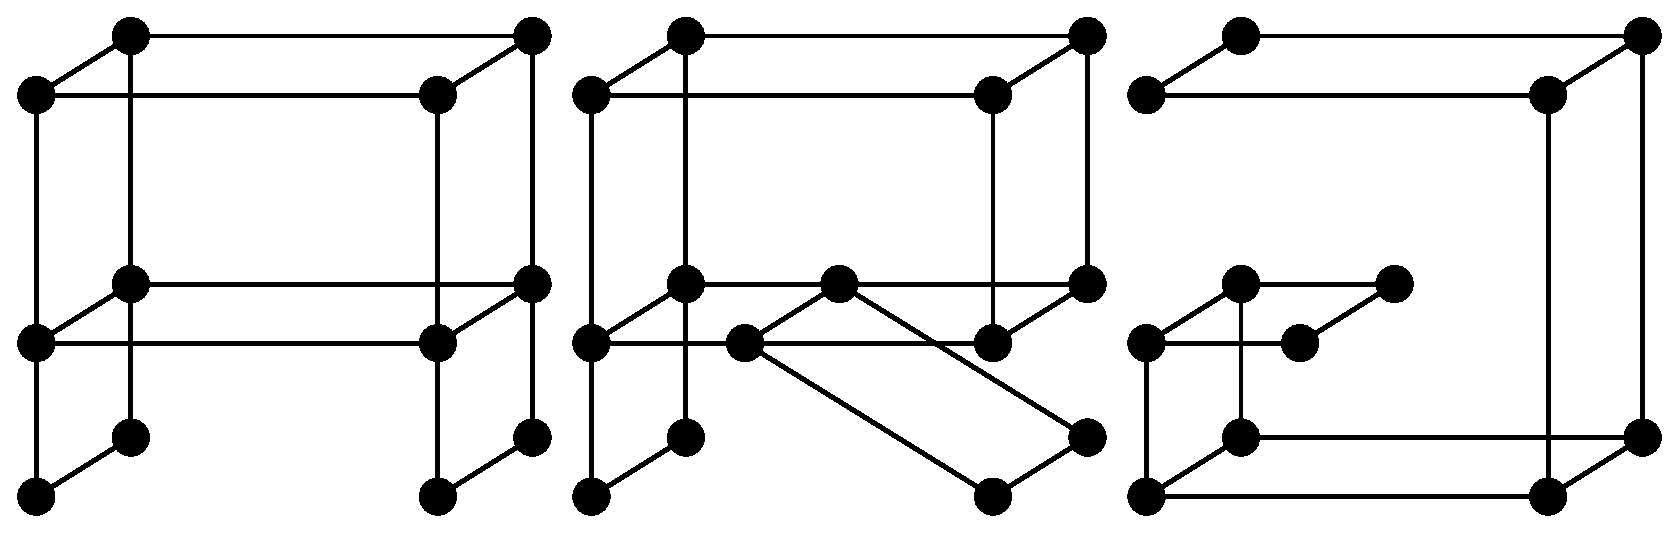
\includegraphics[width=.23\paperwidth]{arg.eps}}

\begin{frame}
  \titlepage
\end{frame}

\logo{}

\begin{frame}
  \frametitle{Sumário}
  \tableofcontents[hideallsubsections]
\end{frame}

\section{Introdução}

\subsection{Algoritmos aleatorizados}

\begin{frame}
  \frametitle{Máquinas de Turing}
  \vspace*{\stretch{1.618034}}
  \begin{center}
    \noindent
    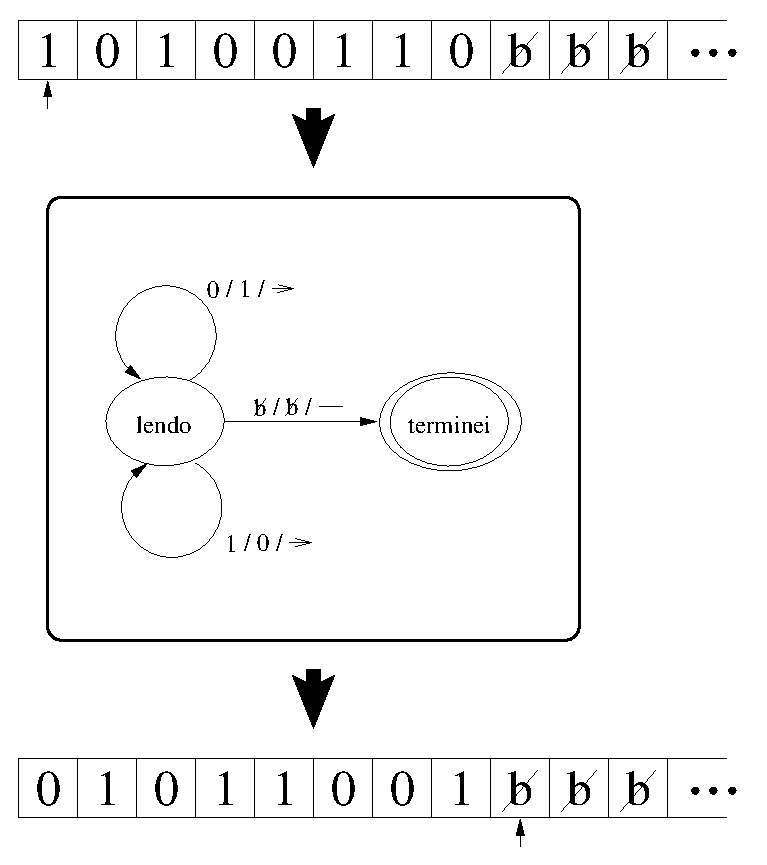
\includegraphics[height=.85\textheight]{turing.eps}
  \end{center}
  \vspace*{\stretch{2.618034}}
\end{frame}

\begin{frame}
  \frametitle{Nomenclaturas sobre máquinas de Turing}
  \vspace*{\stretch{1.618034}}
  \small
  \begin{Nom}<1->[Tempo]
    O \alert{tempo} de uma execução de uma
    máquina de Turing é o número de transições que
    ocorrem durante toda aquela execução.
  \end{Nom}
  \vfill
  \begin{Nom}<2->[Máquina de Turing polinomialmente executável]
    Uma \alert{máquina de Turing polinomialmente executável} é uma
    máquina de Turing que pode ser executada em tempo polinomial no
    tamanho da entrada.
  \end{Nom}
  \vfill
  \begin{Nom}<3->[Determinismo das máquinas de Turing]
    Dizemos que uma máquina de Turing é \alert{determinística}, porque,
    para uma mesma entrada, obtemos sempre o mesmo comportamento da
    máquina.
  \end{Nom}
  \vspace*{\stretch{2.618034}}
\end{frame}

\begin{frame}
  \frametitle{Máquinas de Turing probabilísticas \textit{offline}}
  \vspace*{\stretch{1.618034}}
  \begin{center}
    \noindent
    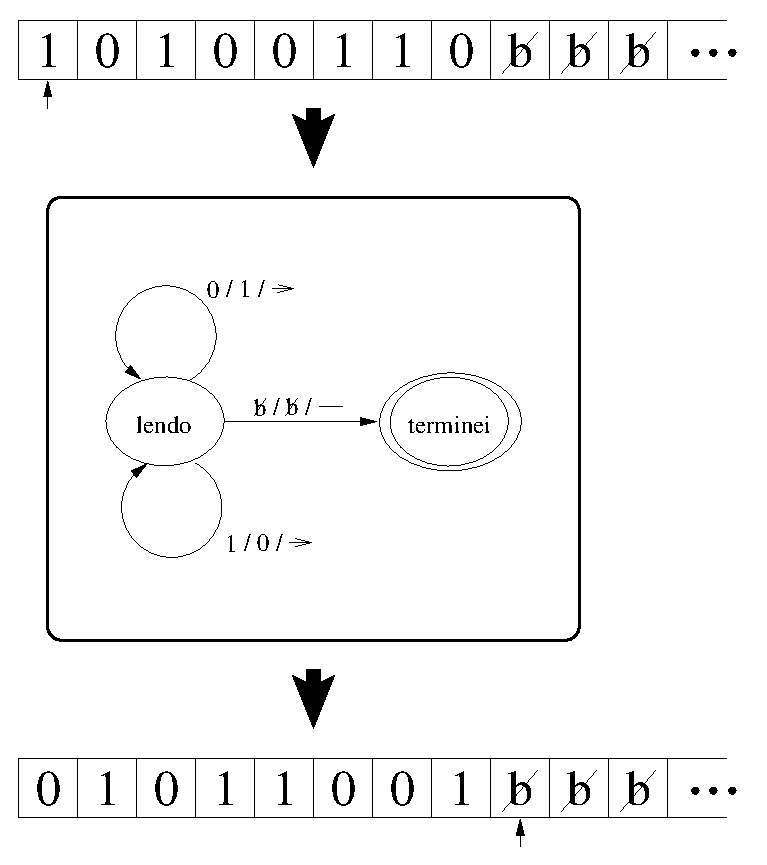
\includegraphics[height=.85\textheight]{turing.eps}
  \end{center}
  \vspace*{\stretch{2.618034}}
\end{frame}

\begin{frame}
  \frametitle{Primalidade}
  \vspace*{\stretch{1.618034}}
  \footnotesize
  \begin{Ex}[Teste de primalidade]
    O algoritmo de Miller-Rabin usa uma sequencia de $m$
    \textit{bits}
    aleatórios para determinar se um número $n$ é primo.
    \begin{itemize}
    \item $n$ primo $\Longrightarrow$ $MR(n)=$ \texttt{primo} sempre.
    \item $n$ composto $\Longrightarrow$ $MR(n)=$ \texttt{primo} com
      probabilidade menor que $\frac14$.
    \end{itemize}
  \end{Ex}
  \pause\vfill
  \begin{equation*}
    \Prob[\text{Miller-Rabin errar para um número menor que $L$}] <
    1\Bigl(\frac{\pi(L)}{L}\Bigr) +
    \frac14\Bigl(1-\frac{\pi(L)}{L}\Bigr)\MMp
  \end{equation*}
  \pause\vfill
  \begin{Teo}[Teorema dos números primos]
    \begin{equation*}
      \pi(L)\sim \textstyle\frac{L}{\ln L}\MMp
    \end{equation*}
  \end{Teo}
  \pause\vfill
  \begin{equation*}
    \Prob[\text{Miller-Rabin errar}] < \frac14\MMp
  \end{equation*}
  \vspace*{\stretch{2.618034}}
\end{frame}

\begin{frame}
  \frametitle{Iteração do teste de primalidade de Miller-Rabin}
  \vspace*{\stretch{1.618034}}
  \begin{block}<1->{}
    Iterando o algoritmo $k$ vezes e garantindo
    a independência entre as sequências de \textit{bits}
    aleatórios, a
    probabilidade de erro no voto da maioria fica menor que
    \begin{equation*}
      {\Bigl(\frac14\Bigr)}^k\MMp
    \end{equation*}
  \end{block}
  \vfill
  \begin{Obs}<2->
    Precisamos de $km$ \textit{bits}
    aleatórios para o procedimento acima. A \alert{Pseudoaleatoriedade}
    trata sobre como gerar $k$ sequências de $m$ \textit{bits} a partir
    de menos que $km$ \textit{bits} aleatórios, de modo que todos
    ``pareçam'' aleatórios. Tal processo é chamado de
    \alert{``reciclagem de
    \textit{bits} aleatórios''}.
  \end{Obs}
  \vspace*{\stretch{2.618034}}
\end{frame}

\section{Aleatoriedade}

\subsection{Distribuições de probabilidades}

\begin{frame}
  \frametitle{Variáveis aleatórias}
  \vspace*{\stretch{1.618034}}
  \begin{Expr}[Paridade do resultado dum lançamento dum dado]
    Seja $S = \{$\textsc{par}$,$\textsc{ímpar}$\}$.\\[12pt]
    \begin{tabular}{lcccccc}
      $\Omega$ &
      \includegraphics[width=.05\paperwidth]{dado1.eps} &
      \includegraphics[width=.05\paperwidth]{dado2.eps} &
      \includegraphics[width=.05\paperwidth]{dado3.eps} &
      \includegraphics[width=.05\paperwidth]{dado4.eps} &
      \includegraphics[width=.05\paperwidth]{dado5.eps} &
      \includegraphics[width=.05\paperwidth]{dado6.eps} \\[12pt]\pause
      $\Omega\rightarrow[0,1]$ &
      $\frac16$ & $\frac16$ & $\frac16$ & $\frac16$ & $\frac16$ &
      $\frac16$ \\[12pt]\pause
      $\funcao{X}{\Omega}{S}$ &
      \textsc{par} & \textsc{ímpar} &
      \textsc{par} & \textsc{ímpar} &
      \textsc{par} & \textsc{ímpar}
    \end{tabular}
  \end{Expr}
  \vspace*{\stretch{2.618034}}
\end{frame}

\begin{frame}
  \frametitle{Construção de espaços de probabilidades sobre variáveis
    aleatórias}
  \vspace*{\stretch{1.618034}}
  \begin{Expr}[Paridade do resultado dum lançamento dum dado]
    \begin{tabular}{lcc}
      \alert{$\Omega_X=S$} &
      \textsc{par} & \textsc{ímpar} \\\pause
      \alert{$\Prob_X=S\rightarrow [0,1]$} &\pause
      $\Prob(2)+\Prob(4)+\Prob(6)=
      \frac16+\frac16+\frac16=\frac12$ &\pause
      $\frac12$
    \end{tabular}
  \end{Expr}
  \vspace*{\stretch{2.618034}}
\end{frame}

\begin{frame}
  \frametitle{Um exemplo de distribuição de probabilidades}
  \vspace*{\stretch{1.618034}}
  \begin{Ex}[Distribuição uniforme]
    \begin{equation*}
      \vetor u =
      \Bigl(\overbrace{\frac1{\cardi{S}},
        \frac1{\cardi{S}},\dotsc,\frac1{\cardi{S}}}^{
        \text{$\cardi{S}$ posições}
      }\Bigr)\MMp
    \end{equation*}
  \end{Ex}
  \vspace*{\stretch{2.618034}}
\end{frame}

\section{Pseudoaleatoriedade}

\subsection{Passeios aleatórios em grafos completos}

\begin{frame}
  \frametitle{Uma analogia imediata}
  \vspace*{\stretch{1.618034}}
  \begin{Obs}<1->
    Uma sequência de $m$ \textit{bits}
    aleatórios pode ser entendida como um
    número em $[0..n-1]$, sendo $n=2^m$. Por exemplo,
    $\text{\texttt{1010}}\mapsto 10$. \pause
    Assim, já que as $k$ sequências $R_1,\dotsc,R_k$
    são independentes, estando na
    $j$-ésima sequência (ou $j$-ésimo número)
    e indo para a $(j+1)$-ésima,
    temos $n$ possibilidades, cada uma com $\Prob=\frac1n$.
  \end{Obs}
  \vfill\pause
  \parbox{.4\linewidth}{
    \centering
    \includegraphics[height=0.3\paperheight]{k8.eps}
  }\hfill
  \parbox{.5\linewidth}{
    $v_0, v_1, \dotsc, v_k \mapsto R_1,\dotsc,R_k$\pause
    \begin{description}
    \item[TOTAL] $km$;\pause
    \item[Ideia] Trocar $m$ por $d$.
    \end{description}
  }
  \vspace*{\stretch{2.618034}}
\end{frame}

\subsection{Passeios aleatórios em grafos regulares}

\begin{frame}
  \frametitle{Troca de grafos completos por grafos regulares}
  \vspace*{\stretch{1.618034}}
  \begin{block}<1->{}
    $G$:
    \begin{itemize}
    \item conexo;\pause
    \item com $n=2^m$ vértices;\pause
    \item bipartido;\pause
    \item $d$-regular;\pause
    \item com todos os laços ($d$ não conta laços);\pause
    \item com a seguinte distribuição de probabilidades para as arestas:
      \begin{description}
      \item[laço] $\frac12$;
      \item[outras arestas] $\frac1{2d}$.
      \end{description}
    \end{itemize}
  \end{block}
  \vspace*{\stretch{2.618034}}
\end{frame}

\begin{frame}
  \frametitle{Exemplo de grafo regular}
  \vspace*{\stretch{1.618034}}
  \begin{center}
    \noindent
    \includegraphics[height=0.8\textheight]{d2p.eps}
  \end{center}
  \vspace*{\stretch{2.618034}}
\end{frame}

\begin{frame}
  \frametitle{Matrizes associadas a $G$}
  \vspace*{\stretch{1.618034}}
  \footnotesize
  \begin{Def}<1->[Matriz de adjacências]
    \begin{equation*}
      {\bigl({\matriz A}_G\bigr)}_{i,j} = \left\{
        \begin{aligned}
          &1, &\quad &\text{se $i$ é adjacente a $j$;}\\
          &0, &\quad &\text{caso contrário.}
        \end{aligned}
      \right.
    \end{equation*}
  \end{Def}
  \vfill
  \begin{Obs}<2->
    Note que, como $G$ possui todos os laços,
    ${\bigl({\matriz A}_G\bigr)}_{i,i}=1$, para todo $i$.
  \end{Obs}
  \vfill
  \begin{Def}<3->[Matriz de transição da cadeia de Markov]
    \begin{equation*}
      {\bigl({\matriz P}_G\bigr)}_{i,j} = \left\{
        \begin{aligned}
          &\frac12, &\quad &\text{se $i=j$;}\\
          &\frac1{2d}, &\quad &\text{se $i$ é adjacente a $j$, mas
            $i\neq j$;}\\
          &0, &\quad &\text{caso contrário.}
        \end{aligned}
      \right.
    \end{equation*}
  \end{Def}
  \vspace*{\stretch{2.618034}}
\end{frame}

\begin{frame}
  \frametitle{Passeios aleatórios do ponto de vista probabilístico}
  \vspace*{\stretch{1.618034}}
  \begin{Obs}<1->
    O passeio aleatório em $G$
    pode ser entendido como uma sequência
    de distribuições de probabilidade.
    \begin{equation*}
      \begin{aligned}
        {\vetor \pi}^{(0)} &=
        \text{distribuição de probabilidades
          inicial}\MMpv\\
        {\vetor \pi}^{(k)} &= {\bigl({\matriz P}_G\bigr)}^k
        \transp{\bigl({{\vetor \pi}^{(0)}}\bigr)}\MMp
      \end{aligned}
    \end{equation*}
  \end{Obs}
  \vfill\pause
  \parbox{.3\linewidth}{
    \begin{equation*}
      \begin{pmatrix}
        \textstyle\frac12 & \textstyle\frac14 & 0 & \textstyle\frac14
        \\
        \textstyle\frac14 & \textstyle\frac12 & \textstyle\frac14 & 0
        \\
        0 & \textstyle\frac14 & \textstyle\frac12 & \textstyle\frac14
        \\
        \textstyle\frac14 & 0 & \textstyle\frac14 & \textstyle\frac12
    \end{pmatrix}
    \end{equation*}
  }\hfill
  \parbox{.3\linewidth}{
    \centering
    \includegraphics[width=.25\textwidth]{d2p.eps}
  }\hfill
  \parbox{.3\linewidth}{
    \begin{equation*}
      \begin{gathered}
        (1,0,0,0) \\
        \bigl(\textstyle\frac12, \textstyle\frac14, 0,
        \textstyle\frac14\bigr)
        \\
        \bigl(\textstyle\frac38, \textstyle\frac14, \textstyle\frac18,
        \textstyle\frac14\bigr)
      \end{gathered}
    \end{equation*}
  }
  \vspace*{\stretch{2.618034}}
\end{frame}

\begin{frame}
  \frametitle{Autovalores de $\matriz P$}
  \vspace*{\stretch{1.618034}}
  \begin{Teo}<1->
    $\matriz P$
    é simétrica e, portanto, diagonalizável, seus autovalores
    $\lambda_1\geq\dotsb\geq\lambda_n$ são reais, e
    \begin{equation*}
      1 = \lambda_1 > \lambda_2 \geq\dotsb\geq \lambda_n\geq 0\MMp
    \end{equation*}
  \end{Teo}
  \vfill
  \begin{Teo}<2->
    \begin{equation*}
      \norma2{{\vetor \pi}^{(k)}-u} \leq \lambda_2^k\MMp
    \end{equation*}
  \end{Teo}
  \vfill
  \begin{Obs}<3->
    $\lambda_2$ pode ser entendido como uma medida de quão perto de
    $\vetor u$ a distribuição ${\vetor{\pi}}^{(k)}$ é. Quanto menor o
    $\lambda_2$, mais próximo.
  \end{Obs}
  \vspace*{\stretch{2.618034}}
\end{frame}

\subsection{Passeios aleatórios em grafos expansores}

\begin{frame}
  \frametitle{Grafos expansores}
  \vspace*{\stretch{1.618034}}
  \begin{Def}<1->[Grafo expansor]
    Um grafo bipartido conexo
    $H=(X\cup Y, E)$ é \alert{$(n,d,c)$-\alert{expansor}} se:
    \begin{enumerate}
    \item $X=Y=\frac{n}2$;
    \item $H$ é $d$-regular;
    \item para todo $W\subseteq X$,
      \begin{equation*}
        \cardi{\cjpp{(w,y)}{w\in W}} \leq
        \biggl( 1 + c\Bigl(
          1 - \frac{2\cardi{W}}{n}
        \Bigr)\biggr)
        \cardi{W}\MMp
      \end{equation*}
    \end{enumerate}
  \end{Def}
  \vspace*{\stretch{2.618034}}
\end{frame}

\begin{frame}
  \frametitle{Autovalores de ${\matriz A}_G$}
  \vspace*{\stretch{1.618034}}
  \begin{Teo}<1->
    ${\matriz A}_G$
    é simétrica e, portanto, diagonalizável, seus autovalores
    $\mu_1\geq\dotsb\geq\mu_n$ são reais, e
    \begin{equation*}
      \mu_1 = -\mu_n = d
    \end{equation*}
  \end{Teo}
  \vfill
  \begin{Not}<2->
    $\mu$ denota o 2\upo maior autovalor \alert{distinto}
    de ${\matriz
      A}_G$. Note-se que \alert{não necessariamente} $\mu=\mu_2$.
  \end{Not}
  \vspace*{\stretch{2.618034}}
\end{frame}

\begin{frame}
  \frametitle{Algumas propriedades dos grafos expansores}
  \vspace*{\stretch{1.618034}}
  \begin{Def}<1->[Discrepância dos grafos expansores]
    Sendo $A\subseteq X$ e $B\subseteq Y$,
    \begin{equation*}
      \MMD(A,B) =
      \Bigcardi{\cardi{E(A,B)}-\frac{2d\cardi{A}\cardi{B}}%
      {n}}\MMp
    \end{equation*}
  \end{Def}
  \vfill
  \begin{Teo}<2->
    \begin{equation*}
      \MMD(A,B) = \cardi{\mu}\sqrt{\cardi{A}\cardi{B}}\MMp
    \end{equation*}
  \end{Teo}
  \vspace*{\stretch{2.618034}}
\end{frame}

\subsection{Reciclagem de {\itshape bits} aleatórios}

\begin{frame}
  \frametitle{Ideia do algoritmo}
  \vspace*{\stretch{1.618034}}
  \begin{block}<1->{}
    \begin{itemize}
    \item $F$ é o conjunto das sequências de \textit{bits} que fazem a
      máquina falhar. Assumimos que $F<\frac{n}{100}$, $n=2^m$ e
      \begin{equation*}
        {\matriz F}_{i,j} = \left\{
          \begin{aligned}
            &1, &\quad &\text{se $i=j$ e $i\in F$;}\\
            &0, &\quad &\text{caso contrário.}
          \end{aligned}
        \right.
      \end{equation*}\pause
    \item $G$ é um $(n,d,c)$-expansor com adição de laços.\pause
    \item $t$ é um natural tal que $\lambda^t_2<\frac1{10}$.\pause
    \item $R_1$ é um vértice aleatório de $G$ (escolhido
      uniformemente).\pause
    \item Passeio aleatório:
      \begin{equation*}
        R_1\xrightarrow{t\text{ passos}}
        R_2\xrightarrow{t\text{passos}}
        R_3\xrightarrow{}\dotsb\xrightarrow{} R_k\MMp
      \end{equation*}
    \end{itemize}
  \end{block}
  \vspace*{\stretch{2.618034}}
\end{frame}

\begin{frame}
  \frametitle{Cálculo da probabilidade total de falha}
  \vspace*{\stretch{1.618034}}
  \begin{Obs}
    Dada uma distribuição de probabilides $\vetor \pi$ sobre os vértices
    de
    $G$, $\norma1{\matriz F\transp{\vetor \pi}}$ representa a
    probabilidade de uma sequência de \textit{bits} escolhida
    aleatoriamente com distribuição $\vetor\pi$ estar em $F$.
  \end{Obs}
  \vfill\pause
  \begin{equation*}
    \lrnorma1{
      \begin{pmatrix}
        1 & 0 & 0 & 0 \\
        0 & 0 & 0 & 0 \\
        0 & 0 & 1 & 0 \\
        0 & 0 & 0 & 0
      \end{pmatrix}
      \begin{pmatrix}
        \frac13 \\ \frac16 \\ \frac13 \\ \frac16
      \end{pmatrix}
    } = \lrnorma1{
      \begin{pmatrix}
        \frac13 \\ 0 \\ \frac13 \\ 0
      \end{pmatrix}
    }
    = \frac23\MMp
  \end{equation*}
  \vspace*{\stretch{2.618034}}
\end{frame}

\begin{frame}
  \frametitle{O grande teorema}
  \vspace*{\stretch{1.618034}}
  \begin{Lem}<1->
    Para todo vetor $\vetor x$ do $\MMR^n$,
    \begin{equation*}
      \norma2{\matriz F{\bigl({\matriz P}_G\bigr)}^t\transp{\vetor x}}
      \leq \frac15\norma2 x
      \qquad\text{e}\qquad
      \norma2{(\matriz I - \matriz F){\bigl({\matriz P}_G\bigr)}^t\transp{\vetor x}}
      \leq \norma2 x\MMp
    \end{equation*}
  \end{Lem}
  \vfill
  \begin{Teo}
    Dada uma máquina $\clBPP$ que usa $m$ \textit{bits} aleatórios por
    rodada, consegue-se uma probabilidade de erro do voto da maioria no
    máximo $\frac{1}{2^k}$ utilizando $O(m+k)$ \textit{bits} aleatórios
    e
    $O(k)$ rodadas.
  \end{Teo}
  \vspace*{\stretch{2.618034}}
\end{frame}

\begin{frame}
  \frametitle{Esboço de demonstração do teorema (I)}
  \vspace*{\stretch{1.618034}}
  \begin{block}{Demonstração.}
    \footnotesize
    $\Prob[R_1\in F] = \norma1{\matriz F\transp{\vetor{\pi^{(0)}}}}\pause
    \leq \sqrt{n}\norma2{\matriz F\transp{\vetor{\pi^{(0)}}}}\pause
    = \sqrt{n}\norma2{\matriz F\transp{\vetor u}}\pause
    \leq \sqrt{n}\sqrt{\frac{n}{100}\bigl(\frac{1}{n^2}\bigr)}
    = \sqrt{n}\bigl(\frac{1}{10\sqrt n}\bigr) \pause
    \leq \frac15$.\pause

    $\Prob[R_2\in F\vert R_1\notin F]
    = \norma1{\matriz F{\bigl({\matriz P}_G\bigr)}^t(\matriz I-\matriz F)
      \transp{\vetor{\pi^{(0)}}}}\pause
    \leq \sqrt{n}\norma2{\matriz F{\bigl({\matriz P}_G\bigr)}^t(\matriz I-\matriz F)
      \transp{\vetor{\pi^{(0)}}}}\pause
    \leq \frac{\sqrt{n}}5\norma2{(\matriz I-\matriz F)
      \transp{\vetor{\pi^{(0)}}}}\pause
    \leq \frac{\sqrt{n}}5\sqrt{n\bigl(\frac{1}{n^2}\bigr)}
    = \frac{\sqrt{n}}5\bigl(\frac{1}{\sqrt n}\bigr) \pause
    \leq \frac15$.

    $\Prob[R_2\in F\vert R_1\in F]
    = \norma1{\matriz F{\bigl({\matriz P}_G\bigr)}^t\matriz F
      \transp{\vetor{\pi^{(0)}}}}\pause
    \leq \sqrt{n}\norma2{\matriz F{\bigl({\matriz P}_G\bigr)}^t\matriz F
      \transp{\vetor{\pi^{(0)}}}}\pause
    \leq \frac{\sqrt{n}}5\norma2{\matriz F
      \transp{\vetor{\pi^{(0)}}}}\pause
    \leq \frac{\sqrt{n}}5\bigl(\frac{1}{10\sqrt n}\bigr) \pause
    \leq \frac1{50} \leq\frac15$.
  \end{block}
  \vspace*{\stretch{2.618034}}
\end{frame}

\begin{frame}
  \frametitle{Esboço de demonstração do teorema (II)}
  \vspace*{\stretch{1.618034}}
  \begin{dem}
    \small
    Indutivamente, dada uma sequência aleatória de
    ``$(\text{bom},\text{ruim},\dotsc)$'' com no mínimo $\frac{k}2$
    ``ruins'', a probabilidade de $(R_1,\dotsc,R_k)$ casar com essa
    sequência é no máximo ${\bigl(\frac15\bigr)}^{\frac{k}2}$.\pause
    Como há $2^k$ possíveis arranjos
    ``$(\text{bom},\text{ruim},\dotsc)$'',
    a probabilidade de $(R_1,\dotsc,R_k)$ conter no mínimo $\frac{k}2$
    ``ruins'' é no máximo $2^k{\bigl(\frac15\bigr)}^{\frac{k}2}$.\pause
    Logo, a probabilidade de erro no voto da maioria é no máximo
    \begin{equation*}
      \Bigl(\frac2{\sqrt 5}\Bigr)^k\MMp
    \end{equation*}
    \pause Sendo $c$ tal que ${\bigl(\frac{2}{\sqrt 5}\bigr)}^c\leq
    \frac12$, rode a máquina $k'=ck=O(k)$ vezes.
    \pause Para gerar $R_1$, precisamos de $m$ \textit{bits}
    aleatórios. \pause
    Para gerar $R_2,\dotsc,R_k$, precisamos de $O(tdk) = O(k)$
    \textit{bits} aleatórios. \pause
    Portanto, para gerar $R_1,\dotsc,R_k$, precisamos de $O(m+k)$
    \textit{bits} aleatórios.
  \end{dem}
  \vspace*{\stretch{2.618034}}
\end{frame}

\section{Semialeatoriedade}

\subsection{Introdução ao conceito}

\begin{frame}
  \frametitle{Assimetria de grafos}
  \vspace*{\stretch{1.618034}}
  \footnotesize
  \begin{Def}<1->[Grafo assimétrico]
    Dizemos que um grafo
    $G$ é  \alert{assimétrico} se o único automorfismo possível sobre
    $G$ é a identidade.
  \end{Def}
  \vfill
  \includegraphics[width=.2\paperwidth]{simetrico1.eps}
  \quad\pause
  $\begin{matrix}
    1 \mapsto 5 \\
    2 \mapsto 4 \\
    3 \mapsto 3 \\
    4 \mapsto 2 \\
    5 \mapsto 1
  \end{matrix}$
  \quad\pause
  \includegraphics[width=.2\paperwidth]{simetrico2.eps} \hfill\pause
  \includegraphics[width=.2\paperwidth]{assimetrico.eps}
  \vfill
  \begin{Obs}
    A probabilidade de um
    grafo com $n$ vértices tomado aleatoriamente ser assimétrico tende a
    $1$ quando $n$ tende ao infinito.
  \end{Obs}
  \vspace*{\stretch{2.618034}}
\end{frame}

\subsection{Semialeatoriedade em subconjuntos do $\MMZ_n$}

\begin{frame}
  \frametitle{Assimetria de grafos}
  \vspace*{\stretch{1.618034}}
  \begin{Def}[Semialeatoriedade para subconjuntos do $\MMZ_n$]
    Diz-se que um subconjunto $S$ do $\MMZ_n$ é \alert{semialeatório}
    quando $S$ satisfaz alguma --- e, por conseguinte, cada
    uma\footnote{As propriedades são todas equivalentes.} --- das
    propriedades listadas a seguir.
  \end{Def}
  \vspace*{\stretch{2.618034}}
\end{frame}



\begin{frame}
  \frametitle{Notações preliminares}
  \vspace*{\stretch{1.618034}}
  \footnotesize
  Dado um subconjunto $S$ de $\MMZ_n$:
  \begin{Def}<1->[Caracter, função característica ou função indicatória]
    \footnotesize
    É a função
    $\funcao{\chi_S}{\MMZ}{\cj{0,1}}$ tal que $\chi_S(z) = 0$, se
    $z\notin S$, e $\chi_S(z) = 1$, caso contrário.
  \end{Def}
  \vfill
  \begin{Def}<2->[Translado de $S$ por $x$]
    $S+x = \cjpp{s+x}{s\in S}$.
  \end{Def}
  \vfill
  \begin{Def}<3->[Grafo associado a $S$]
    $G_S = \bigl(\MMZ_n,\cjpp{\cj{i,j}}{i+j\in S}\bigr)$.
  \end{Def}
  \begin{Not}<4->
    $\bigl(\foraa x\in X\bigr)\bigl(p(x)\bigr) \Longleftrightarrow
    \cardi{\cjpp{x\in X}{p(x)}} = \cardi{X} - o\bigl(\cardi{X}\bigr)$.
  \end{Not}
  \vspace*{\stretch{2.618034}}
\end{frame}

\begin{frame}
  \frametitle{Propriedades sobre a translação}
  \vspace*{\stretch{1.618034}}
  Um subconjunto $S\subseteq\MMZ_n$ tem a propriedade \dots\ se\dots
  \begin{Propr}<1->[Translação fraca]
    Para quase todo $x\in\MMZ_n$,
    \begin{equation*}
      \cardi{S\cap (S+x)} = \frac{\cardi{S}^2}{n} + o(n)\MMp
    \end{equation*}
  \end{Propr}
  \vfill
  \begin{Propr}<2->[Translação forte]
    Para todo subconjunto $T$ de $\MMZ_n$ e quase todo $x$ em $\MMZ_n$,
    \begin{equation*}
      \cardi{S\cap (T+x)} = \frac{\cardi{S}\cardi{T}}{n} + o(n)\MMp
    \end{equation*}
  \end{Propr}
  \vspace*{\stretch{2.618034}}
\end{frame}

\begin{frame}
  \frametitle{Propriedades sobre o padrão}
  \vspace*{\stretch{1.618034}}
  Um subconjunto $S\subseteq\MMZ_n$ tem a propriedade \dots se\dots
  \begin{Propr}<1->[Padrão-$2$]
    Para quase todo $u_1,u_2\in\MMZ_n$,
    \begin{equation*}
      \sum_{s\in S}\chi_S(x+u_1)\chi_S(x+u_2) =
      \frac{\cardi{S}^2}{n} + o(n)\MMp
    \end{equation*}
  \end{Propr}
  \vfill
  \begin{Propr}<2->[Padrão-$k$]
    Para quase todo $u_1,\dotsc,u_k\in\MMZ_n$,
    \begin{equation*}
      \sum_{s\in S}\prod_{j=1}^k\chi_S(x+u_j) =
      \frac{\cardi{S}^k}{n^{k-1}} + o(n)\MMp
    \end{equation*}
  \end{Propr}
  \vspace*{\stretch{2.618034}}
\end{frame}

\begin{frame}
  \frametitle{Propriedades sobre a representação}
  \vspace*{\stretch{1.618034}}
  \footnotesize
  Um subconjunto $S\subseteq\MMZ_n$ tem a propriedade \dots se\dots
  \begin{Propr}<1->[Representação-$2$]
    \footnotesize
    Para quase todo $x\in\MMZ_n$,
    \begin{equation*}
      \sum_{\substack{u_1,u_2\in S\\u_1+u_2=x}}
      \chi_S(u_1)\chi_S(u_2) =
      \frac{\cardi{S}^2}{n} + o(n)\MMp
    \end{equation*}
  \end{Propr}
  \vfill
  \begin{Propr}<2->[Representação-$k$]
    \footnotesize
    Para quase todo $x\in\MMZ_n$,
    \begin{equation*}
      \sum_{\substack{u_1,\dotsc,u_k\in S\\\sum_{\ell=1}^ku_j=x}}
      \prod_{j=1}^k\chi_S(u_j) =
      \frac{\cardi{S}^k}{n^{k-1}} + o(n)\MMp
    \end{equation*}
  \end{Propr}
  \vspace*{\stretch{2.618034}}
\end{frame}

\begin{frame}
  \frametitle{Mais propriedades}
  \vspace*{\stretch{1.618034}}
  Um subconjunto $S\subseteq\MMZ_n$ tem a propriedade \dots se\dots
  \begin{Propr}<1->[Soma exponencial]
    Para todo $j\in\MMZ_n\setminus\cj{0}$,
    \begin{equation*}
      \sum_{x\in S}\chi_S(x){\MMe}^{\frac{2\MMpi\MMi jx}{n}}=o(n)\MMp
    \end{equation*}
  \end{Propr}
  \vfill
  \begin{Propr}<2->[Grafo semialeatório]
    $G_S$ é semialeatório.
  \end{Propr}
  \vspace*{\stretch{2.618034}}
\end{frame}

\begin{frame}
  \frametitle{Mais propriedades ainda}
  \vspace*{\stretch{1.618034}}
  Um subconjunto $S\subseteq\MMZ_n$ tem a propriedade \dots se\dots
  \begin{Propr}<1->[Ciclo-$2t$]
    \begin{equation*}
      \begin{gathered}
        \sum_{x_1,\dotsc,x_{2t}}\chi_S(x_1+x_2)\chi_S(x_2+x_3)\dotsb
        \chi_S(x_{2t-1}+x_{2t})\chi_S(x_{2t}+x_1) \\
        = s^{2t}+o\bigl((n^{2t}\bigr)\MMp
      \end{gathered}
    \end{equation*}
  \end{Propr}
  \vfill
  \begin{Propr}<2->[Densidade relativa]
    Para todo subconjunto $T$ de $\MMZ_n$,
    \begin{equation*}
      \sum_{x,y\in S}\chi_T(x)\chi_T(y)\chi_S(x+y) =
      \frac{\cardi{S}\cardi{T}^2}{n}+o(n^2)\MMp
    \end{equation*}
  \end{Propr}
  \vspace*{\stretch{2.618034}}
\end{frame}

\section{Conclusão}

\begin{frame}
  \frametitle{O que aprendemos neste seminário}
  \vspace*{\stretch{1.618034}}
  \begin{itemize}
    \item A pseudoaleatoriedade trata sobre como, a partir de algumas
      sequências aleatórias, gerar outras sequências, de modo que
      o conjunto
      de todas as sequências se comporte quase
      como se fosse verdadeiramente
      aleatório para a distribuição uniforme.\pause
    \item Vimos que, dada uma máquina $\clBPP$ que usa $m$
      \textit{bits} aleatórios por
      rodada, consegue-se uma probabilidade de erro do voto da maioria
      no      máximo $\frac{1}{2^k}$ utilizando $O(m+k)$ \textit{bits}
      aleatórios      e      $O(k)$ rodadas.\pause
    \item A semialeatoriedade busca definir propriedades equivalentes
      que sirvam para garantir a representatividade de um elemento de
      uma classe, de acordo com aquilo que é esperado que um elemento
      realmente aleatório daquela classe tenha.
  \end{itemize}
  \vspace*{\stretch{2.618034}}
\end{frame}

\begin{frame}
  \frametitle{Referências}
  \vspace*{\stretch{1.618034}}
  \nocite{Quasi-random-subsets}
  \nocite{Quasi-random-graphs}
  \nocite{Chazelle-2000}
  \bibliographystyle{apresentacao}
  \bibliography{apresentacao}
  \vspace*{\stretch{2.618034}}
\end{frame}

\begin{frame}
  \frametitle{}
  \vspace*{\stretch{2.618034}}
  \hfill
  \parbox{.618034\linewidth}{
    \slshape
    Se te parece que sabes e entendes bem muitas coisas, lembra-te que é
    muito mais o que ignoras.

    \begin{flushright}
      \upshape
      (Imitação de Cristo)
    \end{flushright}
  }
  \vspace*{\stretch{1.618034}}
\end{frame}

\end{document}
